% !TeX spellcheck = en_US
\documentclass[11pt, a4paper]{article}
\usepackage[utf8]{inputenc}

\usepackage{latexsym}
\usepackage{float}
\usepackage[utf8]{inputenc}
\usepackage[english]{babel}
\usepackage{microtype}
\usepackage[hyphens]{url}
\usepackage{hyperref}
\usepackage{graphicx}
\usepackage[nonumberlist,acronym]{glossaries}
\usepackage{makeidx}
\usepackage{datetime}
\usepackage{multicol}
\usepackage{setspace}
\usepackage{pdflscape}
\usepackage{pgffor}
\usepackage{enumerate}
\usepackage{booktabs}
\usepackage{tabularx}
\usepackage{braket}
\usepackage{listings}
\usepackage{color}
\usepackage{amsmath}
\usepackage{amssymb}
\usepackage[table,xcdraw]{xcolor}
\usepackage{graphicx}
\usepackage{listings}
\usepackage{hyperref}
\usepackage{vmargin}
\usepackage{wrapfig}
\usepackage{subfiles}
\usepackage{float}
\usepackage{amsmath}
\usepackage{amssymb}
\usepackage{tikz-cd}
\usepackage{multirow}
\usepackage{pgffor}
\usepackage{enumitem}
\usepackage{iflang}
\usepackage{varioref}
\usepackage{hyperref}
\usepackage{cleveref}
\usepackage[justification=centering]{caption}
\usepackage{subcaption}
\usepackage{tikz}
\usepackage{enumitem}
\usepackage{xpatch}
\usepackage{refcount}
\usepackage{color}
\usepackage{pdfpages}
\usepackage{array}
\usepackage{eurosym}


%%%%%%%%%%%%%%%%%%%%%%%%%%%%%%%%%%%%%%%
%%%%%%%%%%%% UTIL COMMANDS %%%%%%%%%%%%  

\setcounter{secnumdepth}{4}
\newcommand{\nc}{\newcommand}
\nc{\supindex}{\textsuperscript}
\renewcommand{\baselinestretch}{1.5}
\nc{\myparagraph}[1]{\paragraph{#1}\mbox{}\\}

%%%%%%%%%%%%%%%%%%%%%%%%%%%%%%%%%%%%%%%
%%%%%%%%%%%%% CONFIG FILE %%%%%%%%%%%%%

\nc{\mytitle}{Economic Viability}
\nc{\mysubtitle}{Bayesian Inference}
\nc{\authors}{\textit{Oriol Alàs Cercós}}
\nc{\datetime}{25\supindex{th} of May, 2022}
\nc{\assignatura}{Technological Business Management and Entrepreneurship}
\nc{\professorat}{Josep Escribà Garriga}

% Per separar professors, utilitzar ','
% 	Ex: Maria, Joan, Pere

%%%%%%%%%%%%%%%%%%%%%%%%%%%%%%%%%%%%%%%
%%%%%%%%%%%%%  LANGUAGE   %%%%%%%%%%%%%

\newcommand{\tr}{\IfLanguageName{english}}

%%%%%%%%%%%%%%%%%%%%%%%%%%%%%%%%%%%%%%%
%%%%%%%%%%%%%%%%% MATH %%%%%%%%%%%%%%%%

\nc{\prob}[1]{P({#1})}
\nc{\probl}[2]{P({#1}|{#2})}

%%%%%%%%%%%%%%%%%%%%%%%%%%%%%%%%%%%%%%%
%%%%%%%%%%%%% FUNCTIONS %%%%%%%%%%%%

\nc{\numitems}[1]{\getrefnumber{#1}}
\newcounter{itemcntr}
\AtBeginEnvironment{itemize}{%
	\setcounter{itemcntr}{0}%
	\xapptocmd{\item}{\refstepcounter{itemcntr}}{}{}%
}

%%%%%%%%%%%%%%%%%%%%%%%%%%%%%%%%%%%%%%%
%%%%%%%%%%%%% RADIO BUTTON %%%%%%%%%%%%

\makeatletter
\newcommand*{\radiobutton}{%
	\@ifstar{\@radiobutton0}{\@radiobutton1}%
}
\newcommand*{\@radiobutton}[1]{%
	\begin{tikzpicture}
		\pgfmathsetlengthmacro\radius{height("X")/2}
		\draw[radius=\radius] circle;
		\ifcase#1 \fill[radius=.6*\radius] circle;\fi
	\end{tikzpicture}%
}
\makeatother


%%%%%%%%%%%%%%%%%%%%%%%%%%%%%%%%%%%%%%%
%%%%%%%%%%%%%  %%%%%%%%%%%%


\newcolumntype{S}{>{\centering\arraybackslash}m{1.5em}}

\renewcommand{\tabularxcolumn}[1]{m{#1}} % redefine 'X' to use 'm'
\newcommand{ \titem}[1]{\item \textbf{#1}\quad}


\newcolumntype{P}[1]{>{\centering\arraybackslash}p{#1}}

\setpapersize{A4}

\author{Oriol Alàs Cercós}
\date{29 d'Abril del 2019}

\makeglossaries
\newacronym{rs}{RS}{Remote Sensing}
\newacronym{sar}{SAR}{Synthetic Aperture Radar}
\newacronym{cnn}{CNN}{Convolutional Neural Network}
\newacronym{gan}{GAN}{Generative Adversarial Network}
\newacronym{cgan}{cGAN}{Conditional Generative Adversarial Network}
\newacronym{mcgan}{McGAN}{Multi-spectral Conditional Generative Adversarial Network}
\newacronym{nir}{NIR}{Near Infra Red}
\newacronym{nlp}{NLP}{Natural Language Processing}
\newacronym{psnr}{PSNR}{Peak signal-to-noise ratio}
\newacronym{ssim}{SSIM}{Structural Similarity Index Metric}

\def\contentsname{Índex}
\begin{document}
	
	\definecolor{gray}{rgb}{0.4,0.4,0.4}
	\definecolor{darkblue}{rgb}{0.0,0.0,0.6}
	\definecolor{cyan}{rgb}{0.0,0.6,0.6}
	\lstset{
		basicstyle=\ttfamily,
		columns=fullflexible,
		showstringspaces=false,
		commentstyle=\color{gray}\upshape
	}
	
	\lstdefinelanguage{XML}
	{
		morestring=[b]",
		morestring=[s]{>}{<},
		morecomment=[s]{<?}{?>},
		stringstyle=\color{black},
		identifierstyle=\color{darkblue},
		keywordstyle=\color{cyan},
		morekeywords={xmlns,version,type}% list your attributes here
	}
	
	\begin{titlepage}
		\begin{figure}[htb]
			\begin{center}
				
				\includegraphics[width=5cm]{imgs/udl.png}\\
				
				
				\medskip
				\begin{center}
					
					\huge\textbf{\mytitle}\\
					\bigskip
					\normalsize{\tr{Made by}{Realitzat per:}}
					\\
					\large\textit{\authors}
					\\
					\setlength{\parskip}{1em}
					\normalsize{\tr{Delivery}{Data de lliurament:}}
					\\
					\large{\datetime}
				\end{center}
				
				\vspace*{\stretch{2.0}}
			\end{center}
		\end{figure}
		\begin{flushright}
			Universitat de Lleida
			\\
			Escola Politècnica Superior
			\\
			Màster en Enginyeria Informàtica
			\\
			\assignatura
			\\
			\medskip
			\textbf{\tr{Professorate:}{Tutor:}}
			\\
			\foreach \n in \professorat{\n\\}
		\end{flushright}
		\thispagestyle{empty} 
	\end{titlepage}
	\pagenumbering{roman}
	\tableofcontents
	\listoffigures
	\listoftables
	\newpage
	\printglossary[type=\acronymtype]
	\newpage
	\pagenumbering{arabic}
	\section{Introduction} 
	\gls{rs} imagery is critical to perform challenges such climate change or natural resources management, including zone monitoring for reforestation, disaster mitigation and land surface change detection.  % canvi de terrenys, natural resources management, climate change, zone monitoring for reforestation, climate change, disaster mitigation 
	Nevertheless, on average 55\% of the Earth's land surfaces is covered by clouds, being then a significant impediment to carry out a broad range of applications. Satellite imagery plagued by films of clouds that obstructs the scene implies a great loss of information or causing effects such as blurring, which mitigates the power of \gls{rs}. Hence, \gls{rs} applications definitely needs a generic technique to detect and remove the cloudy region with an in-painting of the underlying scene.
%	\begin{itemize}
%		\item Generic end-to-end model that can be retrained for specifically ROI by running supplementary iterations but general enough to be great in all geographical locations.
%		\item Free.
%	\end{itemize}
	\subsection{Sentinel2}
	Sentinel2 images are provided by two satellites, Sentinel 2A and Sentinel 2B, which orbit each other with a 180º phase shift. Generally, the acquisition of the images is 10 days per satellite or more or less 5 days altogether. Therefore, a new updated image of a specific area is available in periods of time not exceeding five days. This makes Sentinel-2 data an excellent choice for studying environmental challenges. Sentinel-2 data is multi-spectral with 13 bands in the visible, near-infrared, and short-wave infrared spectrum. These bands come in a different spatial resolution ranging from 10m to 60m, so the images can be classified as medium-high resolution.
	\begin{table}[H]
		\centering
		\caption{Sentinel 2 bands}
		\begin{tabular}{llrrr}
			\hline
			Band & Name                & \parbox{3cm}{\centering \hspace{0.1cm}\\ Central \\ wavelength ($\mu m$) \\ \hspace{0.1cm}} & Bandwidth (nm) & \parbox{3cm}{\centering Spatial\\ resolution (m)} \\ \hline
			B1   & Coastal aerosol     &                      $0.433$ &             27 &                     60 \\
			B2   & Blue                &                        0.490 &             98 &                     10 \\
			B3   & Green               &                        0.560 &             45 &                     10 \\
			B4   & Red                 &                        0.665 &             38 &                     10 \\
			B5   & Vegetation Red Edge &                        0.705 &             19 &                     20 \\
			B6   & Vegetation Red Edge &                        0.740 &             18 &                     20 \\
			B7   & Vegetation Red Edge &                        0.783 &             28 &                     20 \\
			B8   & NIR                 &                        0.842 &            145 &                     10 \\
			B8A  & Vegetation Red Edge &                        0.865 &             33 &                     20 \\
			B9   & Water Vapour        &                        0.945 &             26 &                     60 \\
			B10  & SWIR-Cirrus         &                        1.375 &             75 &                     60 \\
			B11  & SWIR                &                        1.610 &            143 &                     20 \\
			B12  & SWIR                &                        2.190 &            242 &                     20
		\end{tabular}
	\end{table}
% Great indices:
% -  TNDVI - Transformed Normalized Difference Vegetation Index, indicates a relation between the amount of green biomass that is found in a pixel. It has always positive values and the variances of the ratio are proportional to mean values (Senseman et al. 1996).
% Green spectral band was found to be more efficient than the red spectral band to discriminate nitrogen. GNDVI - Green Normalized Difference Vegetation Index (Gitelson et al. 1996) is more sensitive than NDVI to different concentration rates of chlorophyll, which is highly correlated at nitrogen.
% S2REP - Sentinel-2 Red-Edge Position Index is sensitive to both crop (chlorophyll content) N and growth status. Generally, the higher the S2REP value, the higher is the chlorophyll content (Guyot and Baret, 1988). The Sentinel-2 Band 6 (740 nm) measures the reflectance situated at the top of the linear part of the 'red edge' slope.

% Atmospheric reflectance https://www.researchgate.net/publication/340862766_Impact_of_Various_Atmospheric_Corrections_on_Sentinel-2_Land_Cover_Classification_Accuracy_Using_Machine_Learning_Classifiers
	\subsection{Related work and state-of-the-art}
%	Questions:
%	\begin{itemize}
%		\item Cloud detection / Cloud removal
%		\item Which dataset uses?
%		\begin{itemize}
%			\item Bandwidths
%			\item Sparse ROI? How many? Multi-source?
%			\item Pair dataset?
%			\item Multi-Temporal?
%		\end{itemize}
%		\item Model
%		\begin{itemize}
%			\item Fully CNN?
%			\item Residual?
%			\item Needs pair dataset?
%			\item Has a skip connection? Structure of U-Net?
%			\item GAN?
%		\end{itemize}
%		\item Metrics
%	\end{itemize}
	Deep learning have been a popular and efficient technique to solve challenges from satellite imagery. Specifically, \gls{cnn} have been the main architecture of neural networks to provide a solution from image-based problems. 
	\\
	\\
	In \cite{LANARAS2018305}, they create a deep learning approach to Sentinel-2 super-resolution. Their hypothesis was the existence of a complex mixture of correlations across many spectral bands over a large spatial context. Hence, the input of the model is a concatenation of the high-level resolution bands with the low-level resolution bandwidths upsampled to 10m by simple bi-linear interpolations. The model itself is a clear reference of residual networks \cite{he2016deep}. Furthermore, as in ResNet architectures, it uses skip connections to reduce the average effective path length through the network, alleviate the vanishing gradient problem and greatly accelerates the learning during the training.
	\begin{figure}[H]
		\centering
		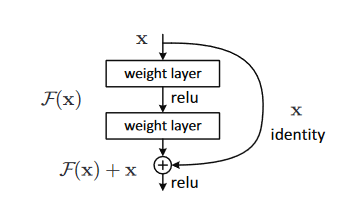
\includegraphics[width=6cm]{imgs/relatedwork/residualblock.png}
		\caption{Residual learning: a building block.}
	\end{figure}
	Similarly, in \cite{Meraner2020}, a residual network is used with the same skip connections mechanism to bring a solution to cloud removal challenge.
	Regarding the design of the neural network, DSen2-CR is a fully convolutional network, so it can accept input images of any spatial dimensions (\textit{m}), as it can be seen in \ref{fig:dsen2-cr}.
	The  output of DSen2-CR is a 13-channel layer, representing the thirteen bands from Sentinel2.  
	\begin{figure}[H]
		\centering
		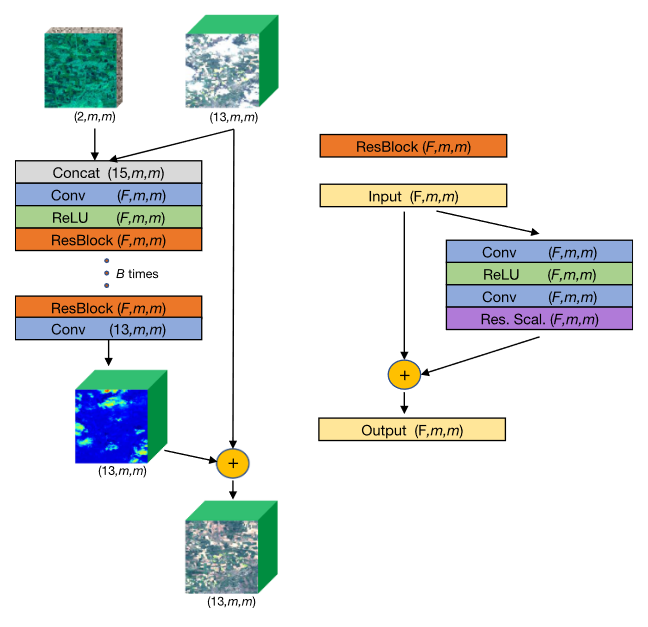
\includegraphics[width=10cm]{imgs/relatedwork/sar.png}
		\caption{DSen2-CR model diagram.}
		\label{fig:dsen2-cr}
	\end{figure}
	 It also uses
	\gls{sar} 
	optical data, which represents an important complementary source to help the model to make greater results. However, \gls{sar} images are affected by a particular type of noise called speckle, which can difficult network's learning. In addition to that, the model depends on one more source to remove the clouds, as \gls{sar} images cannot be downloaded in Sentinel-2. It can be seen in \ref{fig:related-dsen2-cr-predictions} that the lack of \gls{sar} data make the network less powerful. 
	\begin{figure}[H]
		\centering
		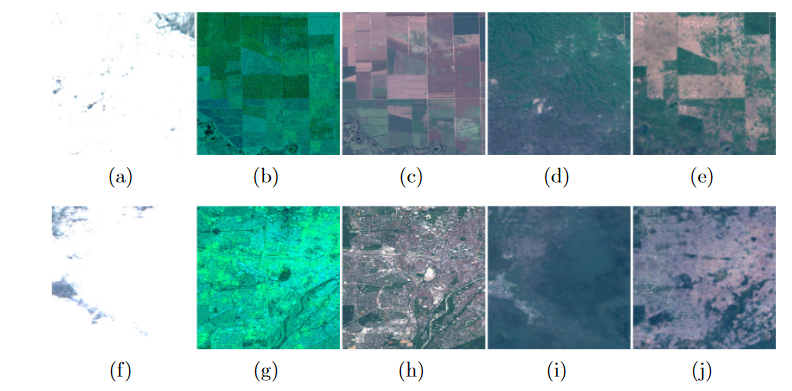
\includegraphics[width=13cm]{imgs/relatedwork/dsen2-cr-predictions.png}
		\caption{Examples of the influence of SAR data. Being (a, f) cloudy images, (b, g), SAR images, (c, h), the target cloudless images, (d, i), the synthesized images without SAR input data and (e, j) the predictions using SAR data as input.}
		\label{fig:related-dsen2-cr-predictions}
	\end{figure}
	Improvements have been found using \gls{gan} \cite{goodfellow2014generative}, which is a model architecture that belongs to the set of generative models. \gls{gan} is an unsupervised model made up of two neural networks: the generator and the discriminator. The idea is based on a game theoretic scenario in which the generator network must compete against an adversary. While the generator network produces samples, the aim of the discriminator is to distinguish between the real samples and the drawn by the generator. The discriminator is a binary classifier trying not to be fooled. The generator loss is calculated using the discriminator as a reference of how much far is from real images while the discriminator loss is calculated by how much accurate is discerning between the synthesized data and the real one. The standard function can be known as the min-max loss:
	\begin{align*}
		Loss_D(D) =& \; E_x[log(D(x)]\\
		Loss_G(G) =& \; E_y[log(1 - D(G(y)))]\\
		Loss_{GAN}(G, D) =&\; Loss_D(D) + Loss_G(G)
	\end{align*}
	During training, both networks constantly try to outsmart each
	other, in a zero-sum game. At some point of the training, the game may end up in a state that
	game theorists call a Nash equilibrium, when no player would be better off changing their own strategy, assuming the other players do not change theirs. \gls{gan}s can only reach one possible Nash equilibrium: when the generator produces so realistic images that the discriminator is forced to guess by 50 \% probability that the image is real or not. Nevertheless, the training process not always can converge to that equilibrium. There are several factors that make the training hard to reach the desired state. For instance, there is a possibility that the discriminator always outsmarts the generator so that it can clearly distinguish between fake and real images. As it never fails, the generator is stuck trying to produce better images as it cannot learn from the errors of the discriminator. Possible solutions can be carried out such as making the discriminator less powerful, decreasing the learning rate or adding noise to the discriminator target. Another big obstacle is when the generator becomes less diverse, and it learns only to perfectly generate realistic images of a single class, so it forgets about the others. This is  called mode collapse. At some point, the discriminator can learn how to beat the generator, but then, the latter is forced to do the same but in another class, cycling between classes never becoming good at any of them. A popular technique to avoid is experience replay, which consists in storing synthetic images at each iteration in a replay buffer. There is a lot of literature of obstacles and solutions to improve \gls{gan} training and it is still very active, as it is in its applications too. The tuning of hyper-parameters and the design of the model will be a key to pursue the Nash equilibrium. For instance, there is a variant called \gls{cgan}. Traditionally, the generative network only produces the image from a random vector as an input, which is also called latent vector since it cannot be manipulated or with prior convictions of how will be. Unfortunately, this only allows to generate a random image from the domain of the latent space, which is hard to map to the generated images. However, \gls{cgan} can be trained so that both generator and discriminator models can be conditioned to some class labels or multi-dimensional vectors and produce synthetic images from a specific domain.
	\\
	\\
	Actually, it is hard to find another \gls{gan} that can fit in cloud removal problem without being \gls{cgan}, since the model needs to be conditioned to the input image. In \cite{8014931}, they %TODO change name
	proposed a  \gls{mcgan} trained using RGB and \gls{nir} cloud-free bands as input and synthetic RBG cloudy images as target. It is true that short wave bands are unaffected by cloud cover and using \gls{nir} images to guide to uncover the clouds of satellite imagery is great since \gls{nir} bands posses have higher penetration through fog than visible light bands. Nevertheless, synthesizing the target might not be realistic enough to feasibly deploy the model in real-state. Regarding the experimental results, they have only showed qualitative metrics by comparing the ground-truth with cloud-free images, ones synthesized and ones real, accompanied both by the cloud obscure image and the cloud mask.  As the NIR channel is not altered by the perlin noise, there is a huge difference about the effectiveness comparing the synthesized images with the real ones, as it can be seen in \ref{fig:related-mcgan-synthesized} and \ref{fig:related-mcgan-real}
	\begin{figure}[H]
		\centering
		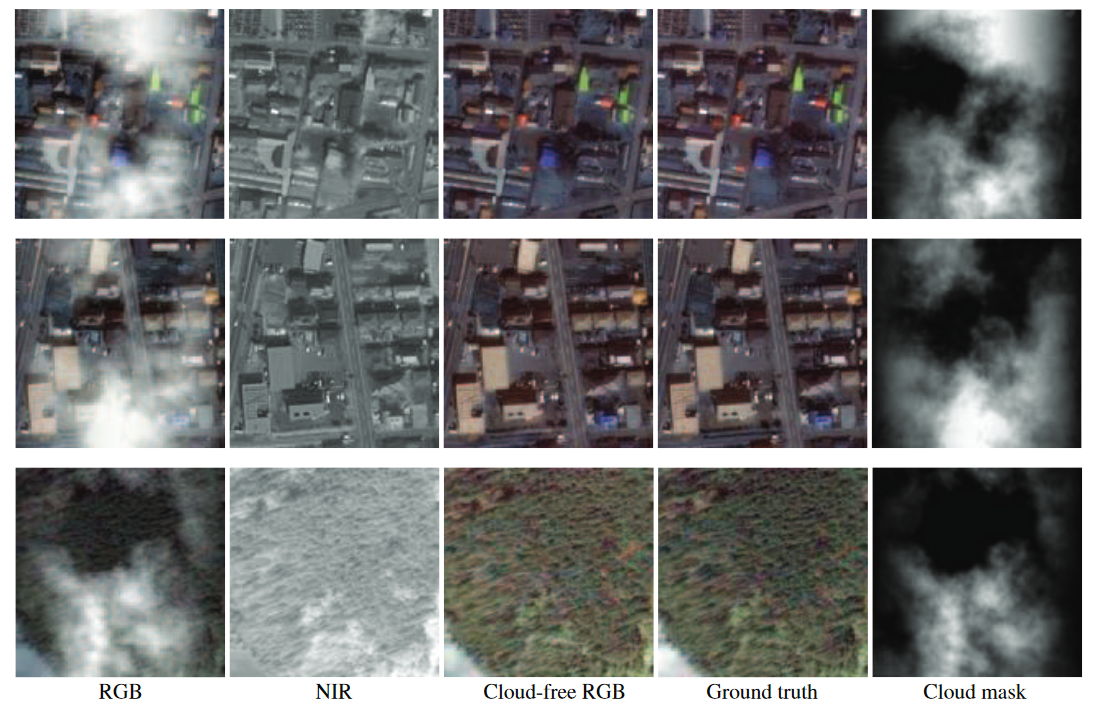
\includegraphics[width=12cm]{imgs/relatedwork/mcgan-synthesized.png}
		\caption{Prediction results by McGAN with the synthesized cloud images}
		\label{fig:related-mcgan-synthesized}
	\end{figure}
	\begin{figure}[H]
	\centering
	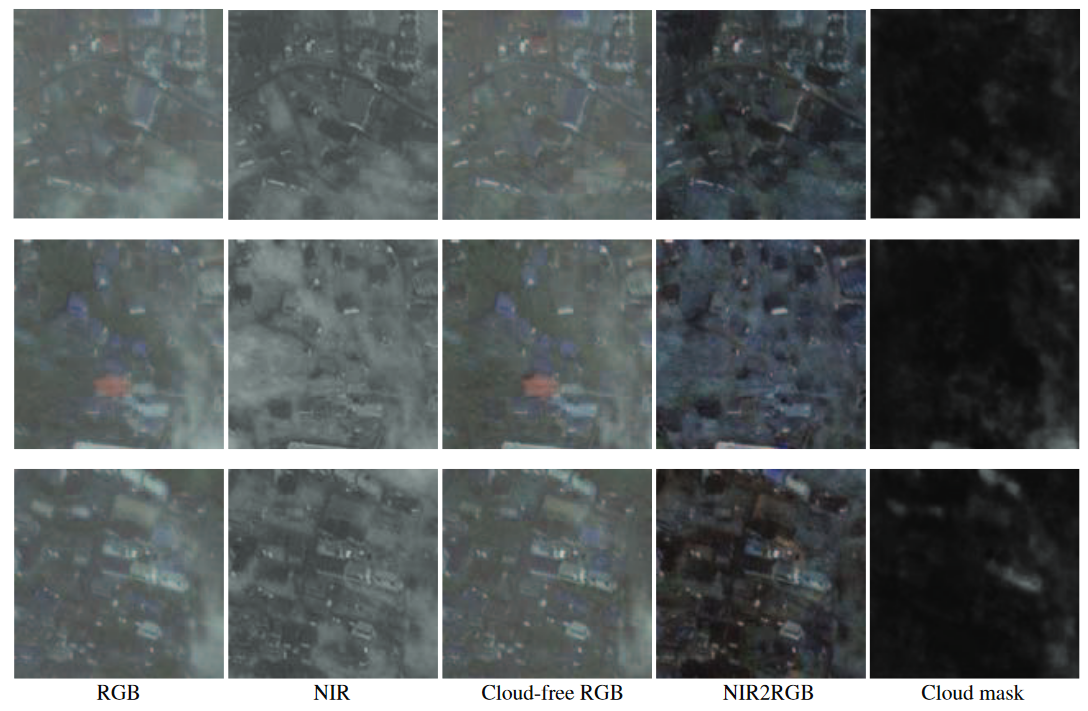
\includegraphics[width=12cm]{imgs/relatedwork/mcgan-real.png}
	\caption{Prediction results by McGAN with the real cloud images}
	\label{fig:related-mcgan-real}
\end{figure}
	To overcome the need of synthesized data, \cite{sarukkai2019cloud} proposed two datasets and two models respective to each of the datasets. Both neural networks have versions depending on including or excluding the \gls{nir} channel as an input. The first is based on Pix2Pix \cite{pix2pix2017} model, a \gls{cgan} which performs very well in image-to-image translation tasks. The generator network of Pix2Pix  uses a encoder-decoder architecture but with skip-connections to avoid loss of information of the bottleneck, similar to U-Net architecture \cite{unet}. The model is trained by a paired dataset of single-images. That means the dataset have a cloudy image as input and a real cloud-free image of the same zone. The generator tries to produce the image as real as the target ones, so it is compulsory to have both images.  The second model proposed is a spatio-temporal \gls{cgan} trained by pairing clear images with three cloudy corresponding from diverse points in time. Instead of only trying the U-Net architecture as in the first model, they have proposed two designs for the generator:
	\begin{itemize}
		\item A branched ResNet generator. It has three encoder-decoder residual networks to learn feature maps from each image, then concatenating their output to learn from these features again and finally, concatenating the result through a final encoder-decoder to generate the new image.
		\item A branched U-Net generator. A slightly modification of the U-Net to allow multiple input images to encode them separately but decoding together and skip connections.
	\end{itemize}
	Moreover, they have also created two paired datasets to train the single-image models and the multi-temporal models respectively to overcome the need of synthesizing the images to make them cloud obscured.
	\\
	\\
	Regarding experimental results, they have compared the single-image model with \gls{mcgan}. On the other hand, they have compared the multi-temporal model with their different versions since it was the first of its kind. The results can be found in \ref{fig:related-cond-single} and \ref{fig:related-cond-multi}. All models from the same comparison were trained using the same datasets created by them. In both cases they have used \gls{psnr} and \gls{ssim} as quantitative metrics and random figure comparison as qualitative metrics. While \gls{psnr} is a pixel-based metric capturing the difference between the corresponding pixels from two images, \gls{ssim} tracks similarity between visible structures and large-scale features in the images.
	\begin{figure}[H]
		\captionsetup{justification=centering}
		\centering
		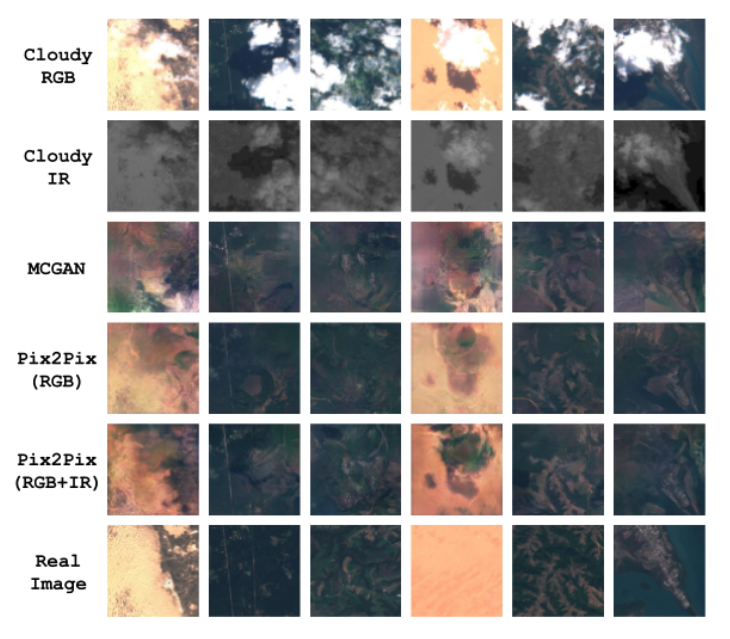
\includegraphics[width=10cm]{imgs/relatedwork/conditional-single-image.png}
		\caption{Comparison between the cloudy images, the outputs of \gls{mcgan} and Pix2Pix-based models and the ground-truth image.}
		\label{fig:related-cond-single}
	\end{figure}
	\begin{figure}[H]
		\captionsetup{justification=centering}
		\centering
		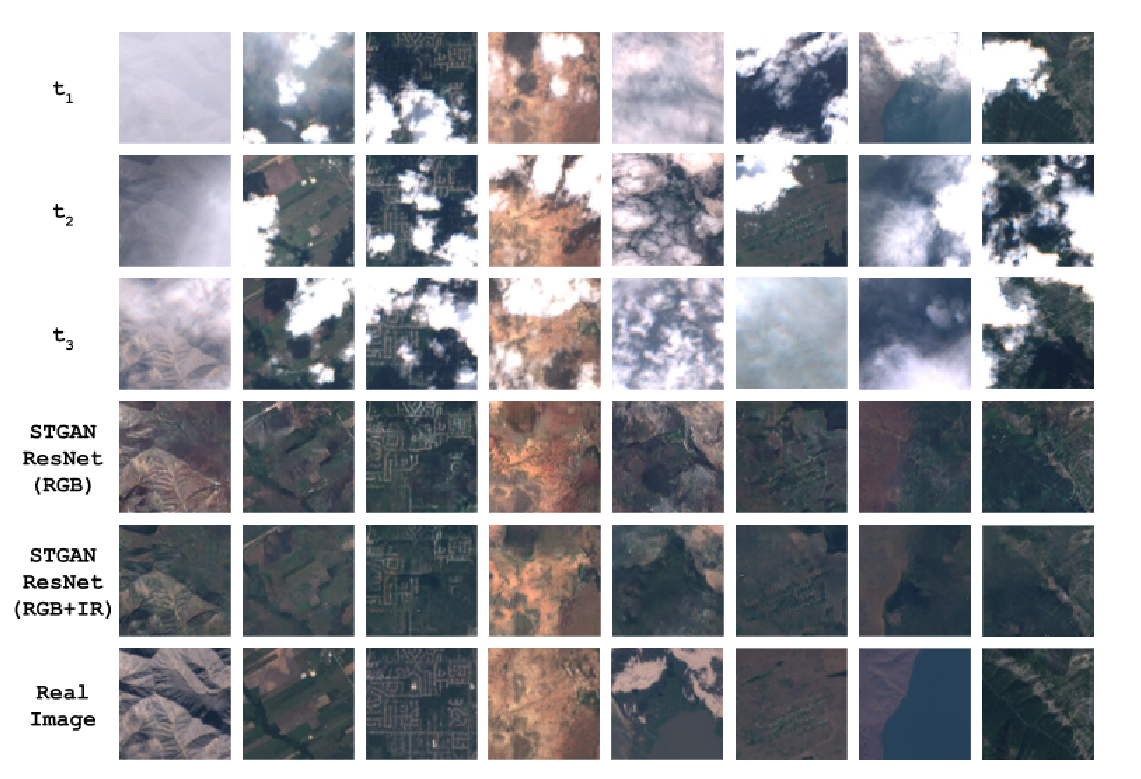
\includegraphics[width=14cm]{imgs/relatedwork/conditional-multi-temporal.png}
		\caption{Comparison between cloudy images, the outputs of \gls{mcgan} versions and the ground-truth image.}
		\label{fig:related-cond-multi}
	\end{figure}
	{
	\renewcommand{\arraystretch}{1.5}%
	\begin{table}[H]
		\caption{PSNR and SSIM of the single-image and multi-temporal model versions .}
		\centering
		\begin{tabular}{l|cccc}
			&\multicolumn{2}{c}{Validation Set}&\multicolumn{2}{c}{Test Set}\\
			\hline\hline
			Model & PSNR & SSIM & PSNR & SSIM\\\hline
			Pix2Pix (RGB) & 23.130 & 0.442 & 22.894 & 0.437\\
			Pix2Pix (RGB + IR)& 21.352 & 0.485& 21.146& 0.481\\
			MCGAN (RGB + IR) & 20.871  & 0.424 & 21.013  & 0.381\\\hline
			STGAN U-Net (RGB) & 25.484 & 0.534 & 25.822 & 0.564\\
			STGAN ResNet (RGB )& 25.519 &  0.550 & 26.000 &  0.573\\
			STGAN U-Net (RGB + IR) & 25.142 & 0.651 & 25.388 &  0.661 \\
			STGAN ResNet (RGB + IR) & 25.628 & 0.724 & 26.186 & 0.734\\\hline
			Raw Cloudy Images & 7.926 & 0.389 & 8.289 & 0.422
		\end{tabular}
	\end{table}
	}
	To overcome the paired-data, Cloud-GAN \cite{cloud-gan} is a Cycle\gls{gan} \cite{CycleGAN2017} which uses two generators ($G_A$ and $G_B$) and two discriminators ($D_A$ and $D_B$). Cycle\gls{gan}s can create new samples of output data, but also transforming the desired data to samples of input data. In essence, they learn to transform data from the two sources by the two generators respectively being also these sources the target. In other words, Cycle\gls{gan} is a model that learns two data transformation functions between two domains. In our case, the generator $G_A$ is generating cloud-free images from cloudy images while the generator $G_B$ is turning the cloud-free images into cloudy. Hence, there is no need to train the model by paired cloudy-cloud-free imagery. The datasets for $G_A$ and $G_b$ are respectively:
	\begin{align*}
		X_A:& \, \{ x \mid x \; \text{is a real cloud obscured image}\}\\
		X_B:& \, \{ x \mid x \; \text{is a real cloud-free image}\}\\
		& \qquad X = X_A \cup X_B
	\end{align*}
	The synthesized data $Y$ can be split into:
	\begin{align*}
		Y_A:& \, \{y \mid y \; \text{is a synthesized cloud obscured image}\}\\
		Y_B:& \, \{y \mid y \; \text{is a synthesized cloud-free image}\}\\
		& \qquad \qquad Y = Y_A \cup Y_B\\
		& 		X_A \cap Y_A = \emptyset, \qquad  X_B \cap Y_B = \emptyset 
	\end{align*}
	The transformation functions from each generator can be expressed as:
	\begin{align*}
		G_A: \text{Generates} \, y \in& \, Y_B \, \text{from} \, z \in Z_A, \qquad Z_A = X_A \cup Y_A\\
		&G_A : Z_A \longrightarrow Y_B\\
		G_B: \text{Generates} \, y \in& \, Y_A \, \text{from} \, z \in Z_B, \qquad Z_B = X_B \cup Y_B\\
		&G_B : Z_B \longrightarrow Y_A
	\end{align*}
	It is well-known that each generator will learn its corresponding transformation function by minimizing the loss, which is calculated by how much the discriminator can discern between their produced data and the real data. On the other hand, the discriminator loss is how good it is to distinguish between the real and the synthesized data.
	\\
	\\
	However, training a cyclic GAN using only the two network losses does not guarantee that cycle consistency is held. Cycle consistency means that given an input, it is desired the back-and-forth transformation $G_B(G_A(z_A)) = z_A'$ to output the the original input $z_A$.  In other words, we want the composition of the transformation functions to be the identity function.
	\[G_A \circ G_B = Id \Longleftrightarrow G_B \circ G_A = Id\]
	Thus, an additional cycle consistency loss is used to enforce this property. This loss is defined as the uniform norm between an input value $z_A$ from the dataset $Z_A$ and it's forward-cycle prediction $G_B(G_A(z_A))$ and the same for the data $z_B \in z_B$, $G_A(G_B(z_B))$. The higher the difference, the more distant the predictions are from the original inputs. Ideally, our network would also minimize this loss by a weighting factor $\lambda$ which is used to control the relevancy of this loss compared to the others.
	\[Loss_{Cycle} = E[G_B(G_A(z_A)) - z_A] + E[G_A(G_B(z_B)) - z_B] \] % TODO: Is x_A or z_A?
	\[Loss_{CycleGAN} = Loss_{GAN}(G_A, D_A) + Loss_{GAN}(G_B, D_B) + \lambda \cdot Loss_{Cycle}\]
	As mentioned before, in \cite{cloud-gan} they did novel deep learning model for cloud removal, since CloudGAN did not need paired-data and they had promising results removing thin clouds, small cloud patches and synthetic clouds. They have great \gls{psnr} in \ref{fig:related-cycle-psnr} although they could only do it for synthetic clouds as the data is not paired, so that there is no quantitative results for real data, neither a comparison with other models proposed. In addition to that, the images to train and test seem to be not diverse enough since they only download satellite images over Paris region.
	\begin{figure}[H]
		\centering
		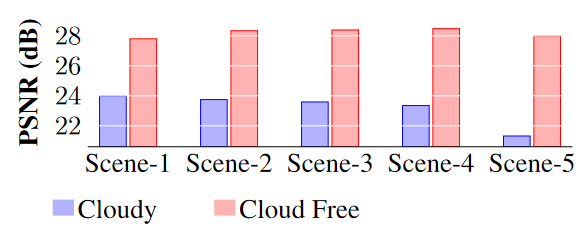
\includegraphics[width=9cm]{imgs/relatedwork/cycle-gan-psnr.png}
		\caption{Failure cases in CloudGAN attempting to removal overly clouded images over-smoothening or completely failing.}
		\label{fig:related-cycle-psnr}
	\end{figure}
	Even though cyclic GANs work excellently to transforming images to different styles, they seemed to be not enough to create new shapes or providing geometric changes as well as they are not general enough providing unexpected results when the input data fed is quite different from the trained. This issue can be also found in Cloud-GAN as its removal cannot be performed well in overly clouded images \ref{fig:related-cloudy-gan-fail}.
	\begin{figure}[H]
		\centering
		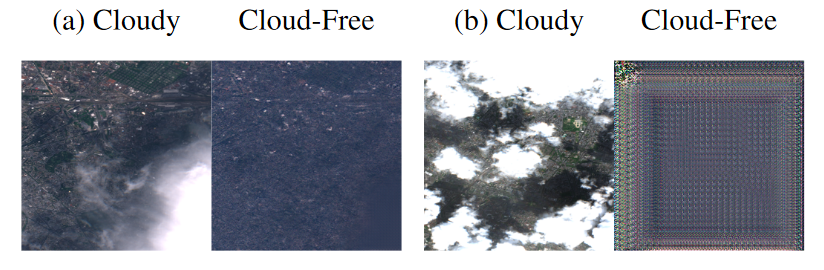
\includegraphics[width=11cm]{imgs/relatedwork/cycle-gan-fail.png}
		\caption{Failure cases in CloudGAN attempting to removal overly clouded images over-smoothening or completely failing.}
		\label{fig:related-cloudy-gan-fail}
	\end{figure}
	Although \gls{cnn} have worked very well for cloud removal, latest and disruptive state-of-the-art deep learning attention-based architectures \cite{VaswaniSPUJGKP17} uncover new paths to achieve remarkable improvements and results. It has been demonstrated that transformers can excellently overcome challenges such \gls{nlp} \cite{brown2020language} 
	, Text-To-Image Generation \cite{pmlr-v139-ramesh21a}  or Image Completion \cite{pmlr-v119-chen20s} with large datasets, great model size and enough compute. Recent contributions have been demonstrated that 
	\section{Data}
	\subsection{Academic Datasets}
	\section{Model architecture}
	
	\section{Experiments \& results}
	\section{Conclusions}
	\section{Bibliography}

	\bibliography{bibliography}
	\bibliographystyle{unsrt}
\end{document}